\DeclareSymbolFont{AMSb}{U}{msb}{m}{n}
\documentclass[11pt,noamsfonts]{amsart}
\usepackage[left=1.5in, right=1.5in, top=1.2in, bottom=1.2in]{geometry}
\usepackage[svgnames]{xcolor}

\usepackage{mathtools}
\usepackage{braket}
\usepackage{enumitem}
\usepackage[charter,expert]{mathdesign}
\usepackage[scaled=.96,osf]{XCharter}% matches the size used in math
\usepackage[tracking]{microtype}
\usepackage{tikz-cd}
\usepackage{stmaryrd}
\usepackage{comment}
\usepackage[scr=esstix]{mathalfa}

\usepackage{caption}
\usepackage{subcaption}

\usepackage{hyperref}
\linespread{1.04}

\usepackage{enumitem}
\setlist[1]{labelindent=\parindent}
\setlist[enumerate]{labelsep=0.5em}
\setlist[enumerate,1]{label={\upshape (\roman*)}, ref={\upshape (\roman*)}}
\setlist[itemize]{label={--}}

\DeclareMathOperator{\Sym}{Sym}

\makeatletter
\let\c@equation\c@section
\let\theequation\thesection
\makeatother

%found on https://tex.stackexchange.com/a/565122 with improvements from TikZ manual:
\tikzset{>={Straight Barb[length=2pt,width=4pt]}, commutative diagrams/arrow style=tikz}

\usepackage[utf8]{inputenc}

\newcommand{\todo}[1]{\footnote{{\sc\color{red}Todo.} #1}}

% Point Formats
\newcommand{\pointheader}{\vspace{2mm}\noindent\refstepcounter{section}\textbf{\thesection.}}
\newcommand{\point}{\pointheader~}
\newcommand{\tpoint}[1]{\pointheader~{\bf #1. ---}}
\newcommand{\epoint}[1]{\pointheader~{\em #1.}}
\newcommand{\bpoint}[1]{\pointheader~{\bf #1.}}

% QED Symbol
\newcommand{\psqedsymb}{\(\blacksquare\)}
\renewcommand{\qed}{~\hfill{\psqedsymb}}


\makeatletter
\newcommand*{\coloneqq}{\mathrel{\rlap{%
           \raisebox{0.3ex}{$\m@th\cdot$}}%
           \raisebox{-0.3ex}{$\m@th\cdot$}}%
           =}
\newcommand{\eqqcolon}{=%
           \mathrel{\rlap{%
           \raisebox{0.3ex}{$\m@th\cdot$}}%
           \raisebox{-0.3ex}{$\m@th\cdot$}}}
\makeatother

\DeclareMathOperator{\Hom}{Hom}
\DeclareMathOperator{\pr}{pr}
\DeclareMathOperator{\op}{op}
\DeclareMathOperator{\id}{id}

% This stuff is for the TikZit diagram
\tikzstyle{none}=[inner sep=0pt]
\tikzstyle{simple}=[-,draw=Black,line width=2.000]
\tikzstyle{arrow}=[-,draw=Black,postaction={decorate},decoration={markings,mark=at position .5 with {\arrow{>}}},line width=2.000]
\tikzstyle{tick}=[-,draw=Black,postaction={decorate},decoration={markings,mark=at position .5 with {\draw (0,-0.1) -- (0,0.1);}},line width=2.000]
\pgfdeclarelayer{edgelayer}
\pgfdeclarelayer{nodelayer}
\pgfsetlayers{edgelayer,nodelayer,main}


\title{Homework for July 22, 2021}
\begin{document}
\maketitle

%\bpoint{Fibre product exercise:}\label{fibre-product-exercise}
%Compare the diagram defining the Cartesian product and the fibre product
%diagrams. Prove that if a category has a terminal object, then the product is a
%fibre product over the terminal object. Prove that a morphism \(Z \to W\) in
%\(\mathcal{C}\) induces a morphism
%\[ X \times_{Z} Y \to X \times_{W} Y. \]
%In particular, if a category has a terminal object, any fibre product maps to
%the Cartesian product.

\tpoint{If a category has a terminal object, then the product is a fibre product over the terminal object}
\begin{proof}
Suppose a category has a terminal object, and binary fibre products.

Let \(X\) and \(Y\) be generic objects in this category. Take the fibre product of \(X\) and \(Y\) over the terminal object. This is an object \( X \times_1 Y \) which will turn out to be the product object,
%We might call this \( X \times_{X \to 1, 1, Y \to 1} Y \) if we were trying to be fully ambiguous or emphasizing that the morphisms are part of the fibre product, but we will usually call it \( X \times_1 Y \)
and a pair of morphisms \(X \times_{1} Y \to X\) and \(X \times_{1} Y \to Y\) which will turn out to be the projections.

%Now we need to use the fibre product's guarantee to establish the product's guarantee.

Suppose there was an object \( Z \) and a pair of morphisms \(Z \to X, Z \to Y \).
%(This is the antecedent of the product definition).
Recall there is a terminal object, \( 1 \). So there are morphisms \( X \to 1, Y \to 1 \) and \( Z \to X ; X \to 1 = Z \to Y ; Y \to 1 = Z \to 1 \). \footnote{Where it is fairly clear from context (because there is only one inhabitant of the type relevant to the argument) we will use types as names, rather than introducing names and then immediately using them only once. So for example \( X \to 1 ; 1 \to 1 = X \to 1 \).}
Recall we are using the semicolon operator for flipped composition of morphisms.

Now we have a commuting square. So by the fibre product property there is a unique morphism \( Z \to X \times_1 Y \), such that \(Z \to X \times_1 Y ; X \times_{1} Y \to X = Z \to X\) and \( Z \to X \times_1 Y ; X \times_{1} Y \to X = Z \to Y \).

% https://tikzcd.yichuanshen.de/#N4Igdg9gJgpgziAXAbVABwnAlgFyxMJZARgBpiBdUkANwEMAbAVxiRAA0ACAHW7wFt4AfWKcAmiAC+pdJlz5CKMgAYqtRizYAtKTJAZseAkWXk19Zq0QddswwqIAmM9QubrE6XfnGlpR+YaViDEUmowUADm8ESgAGYAThD8SGQgOBBIAMxeIInJqdQZSI65+SmIpumZiDl65UhVxYil9UkVac3KZe3ZRTUALD0FLf1IQxSSQA
\begin{tikzcd}
             & Z \arrow[rd] \arrow[ld] \arrow[d] &              \\
X \arrow[rd] & X \times_1 Y \arrow[r] \arrow[l]  & Y \arrow[ld] \\
             & 1                                 &             
\end{tikzcd}

That is, the fibre product over the terminal object is a product.

%We have shown that if a category has a terminal object, and binary fibre products, then it has binary products, constructed as the fibre product over the terminal object.
\end{proof}

\bpoint{Meandering about functors between categories instead of morphisms and objects within one category}
I believe there might be an alternate way of phrasing this, where we talk about several categories and functors between them, instead of objects within a particular category and morphisms between them.

The product, and the fibre product, and many things of this sort in category theory, are universal properties which all have a logical structure, which I attempt to informally gesture at here: for all diagrams A, there exists an extended diagram B, such that among all similar extended diagrams B', B is `best' in some sense.

You can construct the category of functors from a finite discrete two-objects category (let's call this category \(D_2\)) to the category in question (let's call this functor category \( D_2 \to C \)). A particular object of this functor category picks out two objects in the category in question, just like the first part of the universal property of the product.
%\[
%\begin{tikzcd}
%x & y
%\end{tikzcd}
%\]
Similarly, you can take a finite three-objects category with two non-identity arrows pointing from two of the objects at a third object (Let's call this category \( V \)), and construct the category of functors to the category in question (Let's call this functor category \( V \to C \)). A particular object of this functor category picks out two objects with two morphisms to a third shared object, just like the first part of the universal property of the fibre product.
\[
\begin{tikzcd}
x \arrow[r] & z & x \arrow[l]
\end{tikzcd}
\]
The inclusion of the first part of one of these universal properties into the second part corresponds to a particular (injective) functor from one of these finite diagram categories into another finite diagram category. Saying that every antecedent diagram can be completed to a consequent diagram is a map; almost certainly this map should be a functor related to the inclusion functor between the finite diagrams categories. That is, we're considering the product to be an object of the functor category \( (D_2 \to C) \to V^{\op} \to C \). \footnote{As a type-formation operator, and as a sentential logical operator, and as the functor category-formation operator, the rightward arrow associates to the right. \( W \to X \to Y \to Z\) is equivalent to \( W \to (X \to (Y \to Z)) \). Being consistent about this, using the minimum number of parentheses to be unambiguous, is helpful for writing and thinking, in the same way that omitting parentheses in formulas involving binary associative operators is helpful for writing and thinking.}

In order to similarly give an expression for the functor category where the fibre product lives, I need a way to name the finite commutative square category. I think \( 2 \times 2 \) is a reasonable name for it: the product of the category with two objects and one non-identity arrow from one to the other with itself results in a commutative square.

So the fibre product ought to be a nice map from \( V \) shaped diagrams in \( C \) to commuting squares in \( C \), that is, it is an object of the functor category \( (V \to C) \to 2 \times 2 \to C \).

How do I express the compatibility of the product functor \( (D_2 \to C) \to V^{\op} \to C \) with the product inclusion \( D_2 \hookrightarrow V^{\op} \) ?
There's a generic theorem \( B': (A \to B) \to (B \to C) \to A \to C = \lambda x y z . y (x z) \), and so \(B'\) is a reasonable name for the functor that takes functors \( A \to B \) to functors between functor categories \( (B \to C) \to A \to C \).\footnote{Though by the convention previously established, the type expression is itself also an unambiguous name for the functor.}

The inclusion of diagrams \( D_2 \hookrightarrow V^{\op} \) is specified as part of the problem and if we apply \( B' \) to it, we get a functor in the opposite direction to the product functor \( B' (D_2 \hookrightarrow V^{\op}) : (V^{\op} \to C) \to D_2 \to C \). Maybe the way to express the compatibility of the product functor with the product inclusion is to say that if we first apply the product functor, and then do this lifted product inclusion functor back, then we should get the identity. 
\[
(\times) ; B' (D_2 \hookrightarrow V^{\op}) = \id (D_2 \to C)
\]

Similarly, the fibre product \( \times_{X} \) followed by the lifted inclusion of diagrams \( B' (V \hookrightarrow 2 \times 2) : (2 \times 2 \to C) \to V \to C \) should be the identity.
\[
(\times_X) ; B' (V \hookrightarrow 2 \times 2) = \id (V \to C)
\]

From any category, you can take the full subcategory of the objects satisfying some criterion, which is a subcategory. The universal property of both the product and the fibre product is that they are terminal objects in, not the \emph{complete} functor categories corresponding to their types, but in the full subcategory of those functor categories expressing the way that they're compatible with their respective inclusion functors between finite `diagram' categories.

The notation that I'm familiar with is set-builder notation; maybe something like this:

\[
\{ X \in (V \to C) \to 2 \times 2 \to C \mid  
X ; B' (V \hookrightarrow 2 \times 2) = \id (V \to C)
\}
\]

ought to mean something like ``the category consisting of the full subcategory of functors from functors from the V-shaped diagram to the category in question, to functors from the commutative square diagram to the category in question, such that the object composed with the functor resulting from applying the well-known \( B' \) generic functor to the inclusion functor of the V-shaped diagram to the square is equal to the identity on the category of functors from the V-shaped diagram to the category in question''. The fibre product would presumably be the terminal object of this category.

%In this idiom, the idea is to transport a pair of guarantees, that a binary fibre product exists uniquely and a terminal object exists uniquely, into a guarantee that a product exists uniquely.
In order to `move' and `combine' guarantees, like the guarantee that a binary fibre product exists uniquely, I would need lemmas regarding how operations that define categories (such as the functor category construction, the direct product category construction, and the full subcategory construction) interact with guarantees. I think these lemmas might use terms like `preserves' and `reflects' limits and colimits.




\tpoint{A morphism \(Z \to W\) in \(\mathcal{C}\) induces a morphism  \(X \times_{Z} Y \to X \times_{W} Y \)}

\begin{proof}
Given a morphism \(m_1 : Z \to W\), and a fibre product over \(Z\) with morphisms \(m_2 : X \to Z, m_3 : Y \to Z\), and a fibre product over \(W\) with morphisms \(m_4 : X \to W , m_5 : Y \to W\).
 \footnote{Recall we are using the semicolon operator for flipped composition of morphisms}

There already is a commuting square with corners \( X \times_Z Y, X, Y, Z \). We can construct another commuting square, with \(W\) replacing \(Z\) in the corner, using the composed morphisms \( m_2 ; m_1 \) and \( m_3 ; m_1 \).
This commutes because of the associativity of composition. \( X \times_W Y \) is terminal among these commuting squares, and so there is a unique morphism  \(X \times_Z Y \to X \times_W Y \).

% https://tikzcd.yichuanshen.de/#N4Igdg9gJgpgziAXAbVABwnAlgFyxMJZABgBpiBdUkANwEMAbAVxiRAA0ACAHW7wFt4AfQBanAJogAvqXSZc+QigBMpAIxVajFmy68BwgOoTpskBmx4CRACyllm+s1aIQI03MuKiANlIBmR20XEEMPc3krJWQAVnIg5zZJGU8FaxQ1AISdV3ZpTRgoAHN4IlAAMwAnCH4kVRAcCCR-agY6ACMYBgAFSO9XLDBsWBBqJxyQfiE1cKqapDIGpsRMkAZBkKgIHBxC2eraxEXGpBiUkDnD4+Wbc8ukOyW61o6u3q90kEHh1jHgtim-n280QcSeiHqbU6PT6n2+WBGf0SrimymBh1WJ0QtzM92x1CxLTWrxhHyUXyGCN+WmRkyEMXRSExyzOuIOpwJyyJULesPJ8MRNImUxs+SkQA
\begin{tikzcd}
X \times_Z Y \arrow[rrd, dotted] \arrow[rddd] \arrow[rrrrr] &                                                                    &                                       &  &                                  & Y \arrow[ldd, "m_3" description] \arrow[rddd, "m_5" description] &   \\
                                                            &                                                                    & X \times_W Y \arrow[rrru] \arrow[ldd] &  &                                  &                                                                  &   \\
                                                            &                                                                    &                                       &  & Z \arrow[rrd, "m_1" description] &                                                                  &   \\
                                                            & X \arrow[rrru, "m_2" description] \arrow[rrrrr, "m_4" description] &                                       &  &                                  &                                                                  & W
\end{tikzcd}

TODO: I am not sure whether the fibre product over \(W\) is any fibre product over \(W\), as I described above, or whether we are actually talking about \( X \times_{m_2;m_1, W, m_3, m_1} Y \). 
\end{proof}

\tpoint{If a category has a terminal object, any fibre product maps to
the Cartesian product.}

\begin{proof}
Since the fibre product over the terminal object is the Cartesian product, and morphisms of the corner objects induce morphisms of corresponding fibre products, the morphism to from the corner object to the terminal object induces a morphism from any fibre product to the Cartesian product.
\end{proof}

\bpoint{Exercise}\label{monoid-exercise}
Let \(\mathbf{M}\) be a monoid object in \(\mathcal{C}\). Let \(X\) be any other object
in \(\mathcal{C}\) and let \(\mathbf{M}(X) \coloneqq \mathcal{C}(X,\mathbf{M})\) be the
set of arrows from \(X\) to \(\mathbf{M}\) in \(\mathcal{C}\). Verify that \(e\) and \(\mu\)
induce maps \(e(X) \colon \mathbf{1}(X) \to \mathbf{M}(X)\) and \(\mu(X) \colon \mathbf{M}(X) \times \mathbf{M}(X) \to \mathbf{M}(X)\)
and show that \((\mathbf{M}(X), e(X), \mu(X))\) is a monoid in the usual sense.\footnote{Hint: \(\mathbf{1}\) is
a terminal object, so there is a only one map from anything to \(\mathbf{1}\).}

\begin{proof}
Okay, we have a monoidal category - we have finite tensor products of objects,
the tensor product is associative, and there's a terminal object, because it's the tensor product of zero things.

Furthermore, there's a monoid object \(M\). 

There's some generic object \(X\), and we're looking at the set of arrows \(X \to M\).

We want to show that we can use the tensor product of the monoidal category, 
and the way the tensor product is reflected in the monoid object, to give
this set of arrows the structure of a monoid.

\(e X : (X \to 1) \to X \to M\)
\(\mu X : (X \to M) \times (X \to M) \to X \to M\)

What is the candidate for the monoid operation?
We want to use the monoidal category operation, but that takes objects, not arrows.

TODO: not finished


\end{proof}
\tpoint{diagramming}

The \(B'\) combinator has a type \((A \to B) \to (B \to C) \to A \to C\), and a proof \(\lambda x y z .\ y(xz)\). The parse tree of the type, if you unify the nodes representing the generic types \(A, B, C\) can be rearranged to form a fairly reasonable, familiar, triangular diagram of how \(B'\) works. Each of the nodes of the parse tree of the proof has an associated type, and the types are all subformulas of the \(B'\) combinator, and so you can decorate the triangular diagram of the type of \(B'\) with the parse tree of the proof of \(B'\).

\[
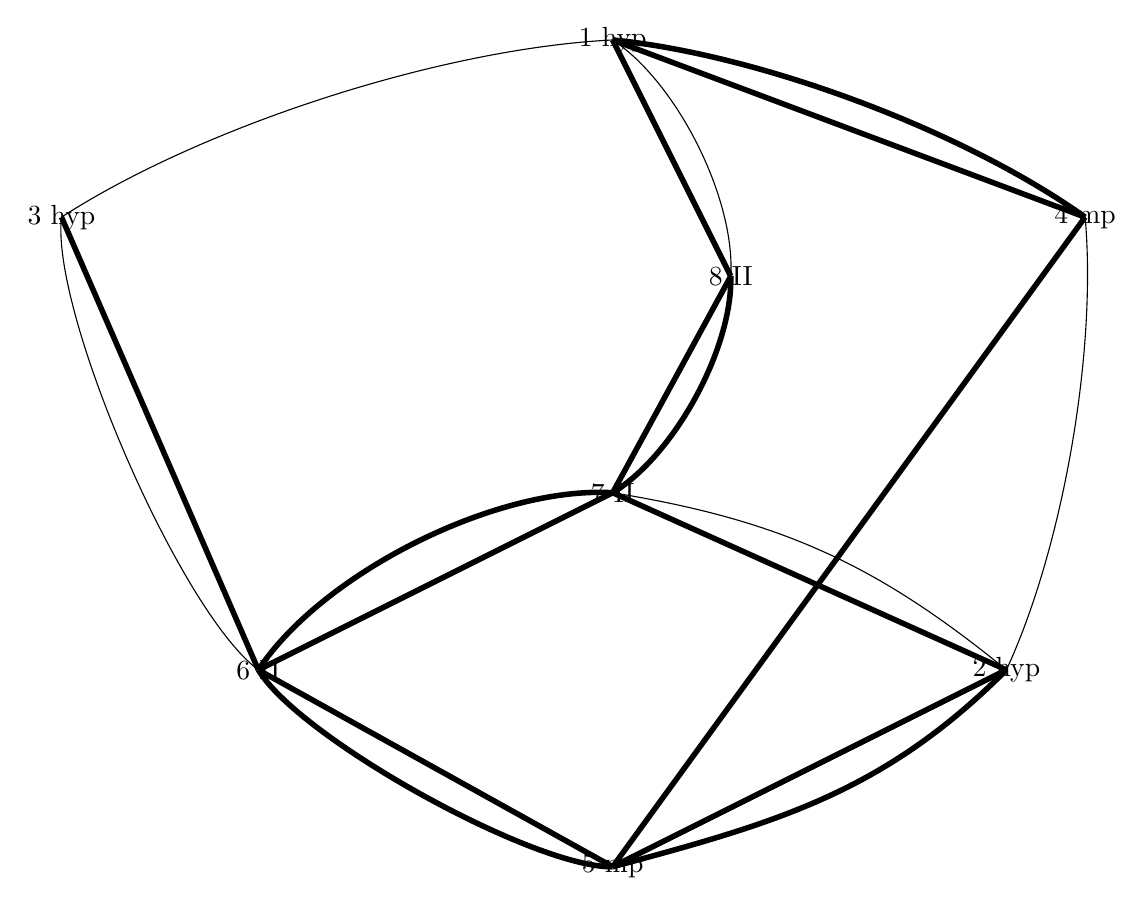
\begin{tikzpicture}
	\begin{pgfonlayer}{nodelayer}
		\node [style=none] (0) at (0, 5.75) {1 hyp};
		\node [style=none] (2) at (5, -2.25) {2 hyp};
		\node [style=none] (4) at (-7, 3.5) {3 hyp};
		\node [style=none] (5) at (6, 3.5) {4 mp};
		\node [style=none] (6) at (0, -4.75) {5 mp};
		\node [style=none] (7) at (-4.5, -2.25) {6 II};
		\node [style=none] (8) at (0, 0) {7 II};
		\node [style=none] (10) at (1.5, 2.75) {8 II};
	\end{pgfonlayer}
	\begin{pgfonlayer}{edgelayer}
		\draw [bend right, looseness=0.50] (4.center) to (7.center);
		\draw [style=simple, bend right, looseness=0.50] (7.center) to (6.center);
		\draw [bend left=15, looseness=0.75] (5.center) to (2.center);
		\draw [style=simple, in=15, out=-135] (2.center) to (6.center);
		\draw [bend right=15] (2.center) to (8.center);
		\draw [style=simple, bend right, looseness=0.75] (8.center) to (7.center);
		\draw [bend left=15, looseness=0.75] (4.center) to (0.center);
		\draw [style=simple, bend left=15, looseness=0.75] (0.center) to (5.center);
		\draw [bend left, looseness=0.75] (0.center) to (10.center);
		\draw [style=simple, bend left, looseness=0.75] (10.center) to (8.center);

		% these are drawn "mp reliance" style, consider adding a style
		\draw [style=simple] (0.center) to (5.center);
		\draw [style=simple] (5.center) to (6.center);
		\draw [style=simple] (2.center) to (6.center);
		\draw [style=simple] (4.center) to (7.center);
		\draw [style=simple] (7.center) to (6.center);
		\draw [style=simple] (8.center) to (7.center);
		\draw [style=simple] (2.center) to (8.center);
		\draw [style=simple] (10.center) to (8.center);
		\draw [style=simple] (10.center) to (0.center);
	\end{pgfonlayer}
\end{tikzpicture}
\]

Ralph Hinze's Concrete Stream Calculus talks about defining integer sequences 

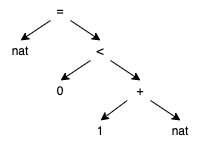
\includegraphics{images/NatStreamParseTree}

\tpoint{Meandering regarding section 6 of Shapely Monads paper}

\bpoint{What is a comma category?} The comma category is a way of constructing a new category by combining two functors to the same category. It generalizes and extends the slice over category constructor, the slice under category constructor, and the arrow category constructor. It combines two functors with the same target. 

If you combine the identity functor with the inclusion functor picking out a particular object using comma, then you get the slice over and under constructors. If you combine the identity functor with itself then you get the arrow category. Combining two inclusion functors using comma results in a category, the objects of which are in bijective correspondence with morphisms from one object to another.


\bpoint{What is a subterminal object?} An object such that every object has at most one morphism into it.

\bpoint{What is a Diers Spectrum?}

Osmond 2012 says:

Spectra have played a prominent role in several regions of mathematics: for instance, 
\begin{itemize}
\item algebraic geometry could resume in some sense as the study of the different flavors of spectra of commutative rings, while 
\item Stone duality is about spectra of distributive lattices and ordered structure; more loosely,
\item categorical model theory is in some sense the study of “spectra of theories”, for a still-to-define notion of 2-dimensional spectra.
\end{itemize} We could sum up the central philosophy behind this notion though
the following claim: spectra arise when free construction fails. A very broad overview of the situation is the following: one starts with a category of algebraic `ambient' objects, and a class of
objects and maps between them one wants to see as `local data', but fails to associate canonically
one local object under an ambient object: one ends up rather with a family of canonical local
objects under an ambient object, which is universal in some sense. The spectrum of an ambient
object is a space whose points index this canonical family under it, equipped with a structural
sheaf whose purpose is to gather those local objects, and it defines a left adjoint to a comparison
functor between categories of `structured spaces'.

What is the category of elements? nlab says it's a way to construct a category from a functor to Set. It's also a comma category \( * \downarrow C \to Set \). It's a special case of something called the Grothendieck construction. 

Definition 3.7 from the Shapely Monads paper says: The `Diers 1978 spectrum' of a small pointwise familial functor 
\(F : \mathcal{A} \to \mathcal{PC}\) is the presheaf \(S_F \in \mathcal{PC}\) given by
\[
SF (c) = \{ t \in y_c \downarrow F : \tilde{t} = t \}
\]
and
\[
S_F (f : d \to c) : t \mapsto \tilde{t y_f}
\]

From nLab Diers Spectrum page: Suppose that \(U: A \to B\)
is a functor that has a left multiadjoint.
The Diers spectrum of \(U\) is the functor
\(B^{\op} \to Set\) that sends an object
\( X \in B \) to the set
\( I \) that indexes the value
\( (g_i : B \to U(A_i))_{i \in I} \)
of the left multiadjoint of \( U \) at
\( X \). A morphism
\( f : X \to X' \) is sent to the induced map \( I' \to I \) that assigns to \( i' \in I' \) the unique \( i \in I \) such that \( g i' \circ f : X \to U( A' i ) \) factors through \( g_i \).


What is a bordage?

What is a Freyd-Kelly factorization system?

What is the Freyd Adjoint Functor Theorem?





\end{document}
